% Options for packages loaded elsewhere
\PassOptionsToPackage{unicode}{hyperref}
\PassOptionsToPackage{hyphens}{url}
%
\documentclass[
  11pt,
]{article}
\usepackage{amsmath,amssymb}
\usepackage{iftex}
\ifPDFTeX
  \usepackage[T1]{fontenc}
  \usepackage[utf8]{inputenc}
  \usepackage{textcomp} % provide euro and other symbols
\else % if luatex or xetex
  \usepackage{unicode-math} % this also loads fontspec
  \defaultfontfeatures{Scale=MatchLowercase}
  \defaultfontfeatures[\rmfamily]{Ligatures=TeX,Scale=1}
\fi
\usepackage{lmodern}
\ifPDFTeX\else
  % xetex/luatex font selection
\fi
% Use upquote if available, for straight quotes in verbatim environments
\IfFileExists{upquote.sty}{\usepackage{upquote}}{}
\IfFileExists{microtype.sty}{% use microtype if available
  \usepackage[]{microtype}
  \UseMicrotypeSet[protrusion]{basicmath} % disable protrusion for tt fonts
}{}
\makeatletter
\@ifundefined{KOMAClassName}{% if non-KOMA class
  \IfFileExists{parskip.sty}{%
    \usepackage{parskip}
  }{% else
    \setlength{\parindent}{0pt}
    \setlength{\parskip}{6pt plus 2pt minus 1pt}}
}{% if KOMA class
  \KOMAoptions{parskip=half}}
\makeatother
\usepackage{xcolor}
\usepackage[a4paper,top=21mm,bottom=19mm,left=21mm,right=21mm]{geometry}
\setlength{\emergencystretch}{3em} % prevent overfull lines
\providecommand{\tightlist}{%
  \setlength{\itemsep}{0pt}\setlength{\parskip}{0pt}}
\setcounter{secnumdepth}{-\maxdimen} % remove section numbering
% Phase 7 original mathematical essay layout
\usepackage{fontspec}
\setmainfont{Noto Serif}
\setsansfont{DejaVu Sans}
\usepackage{amsmath,amssymb,mathtools}
\usepackage{graphicx,float}
\usepackage[most]{tcolorbox}
\usepackage{titlesec}
\usepackage{fancyhdr}
\usepackage{caption}
\usepackage{microtype}
\usepackage{xcolor}
\usepackage{hyperref}
\definecolor{essayink}{HTML}{1E3045}
\definecolor{essayteal}{HTML}{0A9079}
\definecolor{essaymuted}{HTML}{687989}
\definecolor{essayrule}{HTML}{DFE7EC}
\definecolor{essaypale}{HTML}{EAF6F2}
\hypersetup{colorlinks=true,linkcolor=essayteal,urlcolor=essayteal,citecolor=essayteal,
 pdftitle={The Paradox of Absolute Luck: Can Probability Favor Everyone?},
 pdfsubject={Accessible mathematical essay with explicit synthetic thought experiments},
 pdfauthor={Anonymous draft}}
\setlength{\parindent}{0pt}
\setlength{\parskip}{7pt}
\linespread{1.105}
\setcounter{secnumdepth}{0}
\titleformat{\section}{\normalfont\Large\bfseries\color{essayink}}{}{0pt}{}
\titlespacing*{\section}{0pt}{15pt}{4pt}
\captionsetup{labelfont={sf,bf},font={small},justification=raggedright,singlelinecheck=false,skip=3pt}
\pagestyle{fancy}
\fancyhf{}
\fancyhead[L]{\fontsize{8}{10}\selectfont\sffamily\color{essaymuted}ABSOLUTE LUCK  /  MATHEMATICAL ESSAY}
\fancyhead[R]{\fontsize{8}{10}\selectfont\sffamily\color{essaymuted}NOVEMBER 2026}
\fancyfoot[C]{\fontsize{9}{10}\selectfont\sffamily\color{essaymuted}\thepage}
\renewcommand{\headrulewidth}{0.25pt}
\setlength{\headheight}{14pt}
\renewcommand{\maketitle}{%
{\sffamily\fontsize{9}{12}\selectfont\bfseries\color{essayteal}FICTION \quad / \quad PROBABILITY \quad / \quad A MATHEMATICAL INVESTIGATION}\par\vspace{11pt}
{\fontsize{29}{33}\selectfont\bfseries\color{essayink}The Paradox of Absolute Luck}\par\vspace{4pt}
{\fontsize{17}{23}\selectfont\color{essayink}Can probability favor everyone?}\par\vspace{12pt}
{\color{essayrule}\rule{\linewidth}{.9pt}}\vspace{5pt}
}
\ifLuaTeX
  \usepackage{selnolig}  % disable illegal ligatures
\fi
\usepackage{bookmark}
\IfFileExists{xurl.sty}{\usepackage{xurl}}{} % add URL line breaks if available
\urlstyle{same}
\hypersetup{
  pdftitle={The Paradox of Absolute Luck},
  hidelinks,
  pdfcreator={LaTeX via pandoc}}

\title{The Paradox of Absolute Luck}
\author{}
\date{}

\begin{document}
\maketitle

\emph{An original mathematical essay inspired by} Hardcore Leveling
Warrior. \emph{The scenes and numerical experiments below are invented
thought experiments, not measured events from the webtoon.}

\section{The duel with two guaranteed
winners}\label{the-duel-with-two-guaranteed-winners}

Imagine an arena with only one rule: \textbf{exactly one person leaves
victorious}. A mysterious power whispers to Fighter A, ``You have a 99\%
chance of winning.'' Fighter B enters with the same power---and hears
precisely the same promise.

For a moment, both promises sound reasonable. Each fighter is
extraordinarily lucky. But the mathematics has a problem. Let \(W_A\)
mean ``A wins'' and \(W_B\) mean ``B wins.'' Because one victory
excludes the other,

\[P(W_A)+P(W_B)\leq 1.\]

Two simultaneous 99\% promises instead demand \(0.99+0.99=1.98\). It is
tempting to say luck has broken probability. The more interesting answer
is that our \emph{description} of luck is incomplete.
\textbf{Ninety-nine percent against whom? In which contest?}

One possible model gives each competitor a positive strength \(w\). In a
two-person contest, the chance of winning is the player's strength
divided by the two strengths combined:

\[P(A\text{ wins against }B)=\frac{w_A}{w_A+w_B}.\]

Give each lucky fighter strength 99 and an ordinary opponent strength 1.
Either lucky fighter beats the ordinary opponent 99\% of the time.
Against each other, however, they each win 50\% of the time. No
guarantee was broken: the two 99\% statements belonged to
\emph{different matchups}. This is an illustrative use of the
established Bradley--Terry/Luce family of choice models, not a law of
supernatural luck {[}1,2{]}.

Nor must the duel be 50--50. Equal records against an ordinary opponent
do not, by themselves, establish equal chances against each other. The
real lesson is that a winning percentage cannot float free of its
opponent and setting.

\begin{figure}[H]
\centering
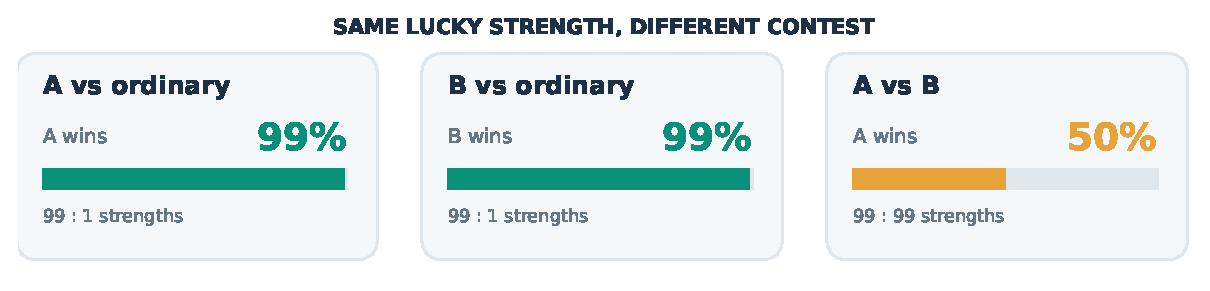
\includegraphics[width=.96\linewidth]{figures/fig01_matchups.pdf}
\caption{Two 99\% outcomes against different opponents do not imply two 99\% winning chances in the same duel.}
\end{figure}

\section{Three coins, and the trap of
independence}\label{three-coins-and-the-trap-of-independence}

Now replace the duel with coins. Suppose each of three coins succeeds
with probability 99.5\% \textbf{while all three are being used
together}. Can the probability that all three succeed drop to 60\%?

Call failure of coin \(i\) the event \(F_i\). For at least one coin to
fail, one of \(F_1,F_2,F_3\) must occur. Even when failures are
dependent, the union bound gives

\[P(F_1\cup F_2\cup F_3)\leq 0.005+0.005+0.005=0.015.\]

So the probability that \emph{all three succeed} is at least
\(1-0.015=98.5\%\). A collective 60\% success rate cannot coexist with
all three \textbf{same-context} marginals remaining at 99.5\% {[}3{]}.
It would require the individual rates to change, or the original
statement to refer to another situation---for example, activating a coin
alone.

The phrase ``almost certain'' is not enough. We need to know whether the
probabilities describe isolated coins, a simultaneous batch, or a
particular relationship among outcomes.

\section{Two hundred coins and no possible perfect
run}\label{two-hundred-coins-and-no-possible-perfect-run}

Now comes the seemingly impossible twist. Increase the number of coins
to \textbf{200}. Imagine 200 equally likely possible worlds. In world 1,
only coin 1 fails. In world 2, only coin 2 fails. Continue this pattern
until world 200, where only coin 200 fails.

Choose a world uniformly at random. Any particular coin fails in exactly
one world out of 200. Therefore,

\[P(\text{coin }i\text{ succeeds})=\frac{199}{200}=99.5\%.\]

But \emph{every} world contains a failure. There is not a single world
in which all 200 coins succeed:

\[\boxed{P(\text{all 200 succeed})=0.}\]

We did not lower the reliability of any coin. We changed \textbf{how
their failures fit together}. In the three-coin example, there were too
few small failure probabilities to cover every possibility. With 200
coins, 200 separate half-percent failure events can exactly cover the
entire probability space.

Independence would tell a completely different story. If the 200 coins
instead succeeded independently with probability 0.995 each, then

\[P(\text{all succeed})=(0.995)^{200}\approx36.70\%.\]

Same 99.5\% for each coin. One model gives 0\% joint success; another
gives approximately 36.70\%. A third mathematically valid
shared-parameter model gives approximately 49.87\%. \textbf{Individual
luck alone cannot determine collective luck.}

\begin{figure}[H]
\centering
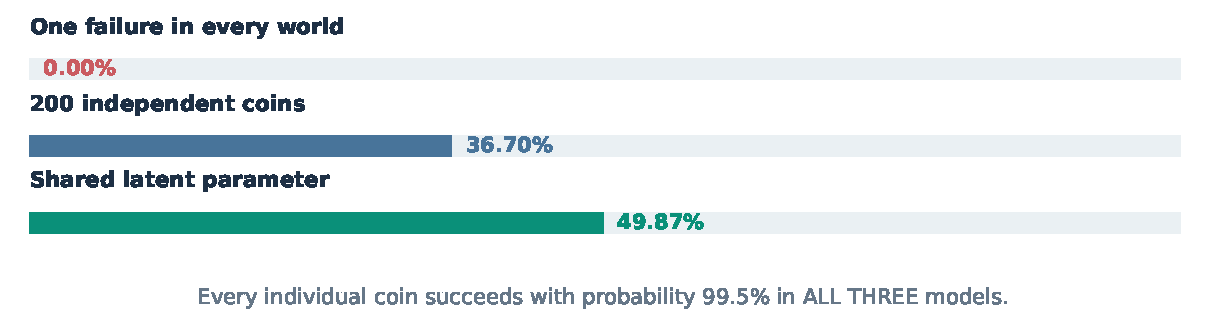
\includegraphics[width=.96\linewidth]{figures/fig03_two_hundred_models.pdf}
\caption{Three exact joint-success probabilities under different stipulated dependence mechanisms; all 200 individual marginals equal 99.5\%.}
\end{figure}

\begin{figure}[H]
\centering
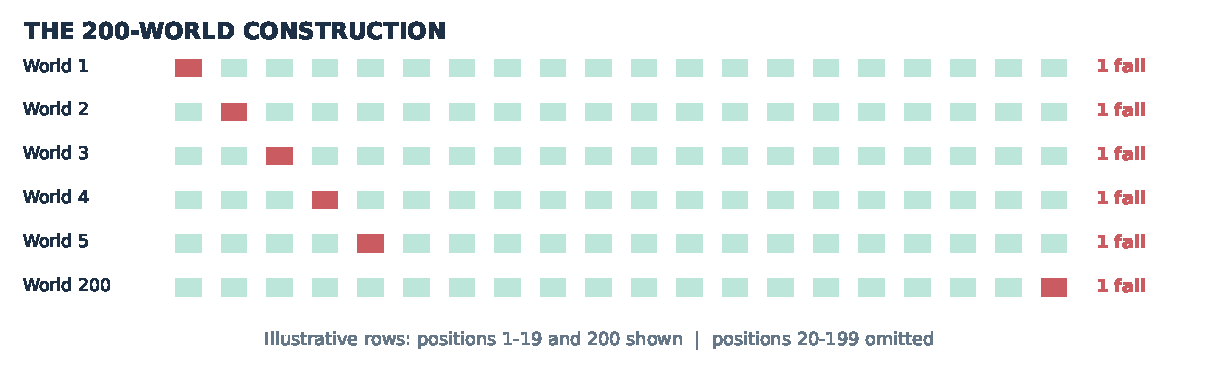
\includegraphics[width=.96\linewidth]{figures/fig02_failure_worlds.pdf}
\caption{Only representative rows and coin positions are pictured; the construction has 200 complete equally likely worlds, with one failure per world.}
\end{figure}

\section{The coin that cannot be
added}\label{the-coin-that-cannot-be-added}

Our zero-success construction is symmetric: swapping coin labels changes
nothing. Mathematicians call this \emph{exchangeability}. Surprisingly,
the exact 200-coin construction cannot be extended to \textbf{201
exchangeable coins} while keeping the original joint law for the first
200 {[}4{]}.

Here is an intuitive way to see why. In any exchangeable 201-coin
extension, \emph{every choice of 200 coins} would have to contain
exactly one failure, with certainty. If all 201 coins contained exactly
one failure, omitting the failed coin would leave none. If they
contained two failures, omitting a successful coin would leave two. Zero
failures or three or more are no better. No arrangement works for every
possible omission.

This does \textbf{not} mean the universe forbids a 201st coin. It means
the exact probability model cannot preserve all of those symmetry
requirements at once. Finite and infinitely extendible probabilistic
models are not interchangeable; that distinction is part of established
exchangeability theory {[}4,5{]}.

\section{The information missing from every
pair}\label{the-information-missing-from-every-pair}

Suppose a researcher watches three coins and finds that each succeeds
70\% of the time, and any chosen pair succeeds together 50\% of the
time. Surely that tells us the chance all three succeed?

Not quite. Construct two models, L and H. Both obey those
\textbf{identical} single-coin and pairwise statistics. Yet model L
gives a 30\% chance of all three succeeding, while model H gives 40\%.

Nothing is wrong with the measurements. They simply do not reveal the
three-way dependence. If observations are restricted to a fresh single
coin or pair on each trial, these two models generate exactly the same
observable data. To distinguish them, one must sometimes see the
\textbf{whole triple from the same trial}.

We often ask whether two things are correlated. Absolute Luck suggests a
subtler question: \emph{What relationships appear only when three or
more things happen together?}

\begin{figure}[H]
\centering
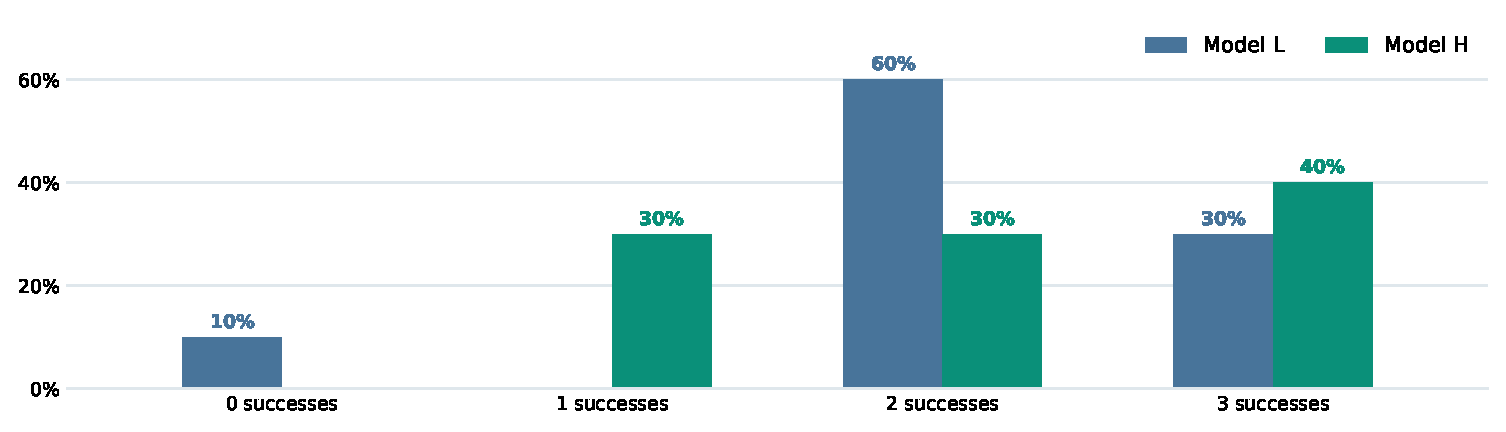
\includegraphics[width=.96\linewidth]{figures/fig04_hidden_triple.pdf}
\caption{Identical single-coin and pairwise probabilities can conceal different distributions of the number of successes.}
\end{figure}

\section{The best use of luck depends on the
rules}\label{the-best-use-of-luck-depends-on-the-rules}

Imagine a limited probability boost of 49.5 percentage points, shared
among three coins that each start at 50\%. We can distribute it equally,
making each coin 66.5\% reliable, or concentrate it on the first coin,
giving probabilities 99.5\%, 50\%, and 50\%.

If outcomes are independent, equal sharing wins when the goal is for
\textbf{all three} to succeed: \(0.665^3\approx29.41\%\), compared with
\(0.995(0.5)(0.5)=24.875\%\).

Now change the dependence rule but \textbf{hold that new rule fixed
across both strategies}. Draw one uniform random number \(U\) between
zero and one. Coin 1 succeeds when \(U\geq1-p_1\); coins 2 and 3 succeed
when \(U\leq p_2\) and \(U\leq p_3\). All individual success rates
remain correct. Yet the equal strategy now yields 33\% collective
success, while concentration yields 49.5\%.

The ranking has reversed. This comparison concerns these two strategies
under an illustrative mechanism; it does \textbf{not} prove
concentration is globally optimal. It shows why an instruction as simple
as ``spread luck evenly'' needs a dependence assumption.

\begin{figure}[H]
\centering
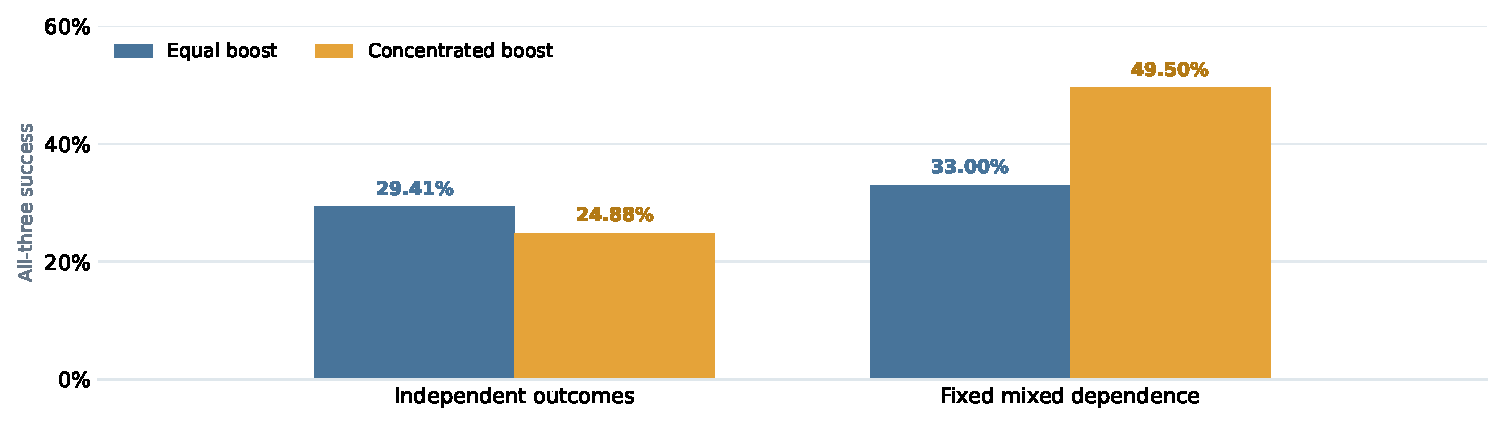
\includegraphics[width=.96\linewidth]{figures/fig05_allocation_reversal.pdf}
\caption{Two allocation strategies reverse their ordering when the joint dependence mechanism changes. Both bars within each setting use the same coupling.}
\end{figure}

\section{What a computer can---and
cannot---prove}\label{what-a-computer-canand-cannotprove}

Our companion mathematical study ran seeded simulations with 120,000
trials per principal scenario and checked them against exact formulas.
For the 200-coin cases, the simulated all-success frequencies were 0\%,
36.57\%, and 49.75\% under three different stipulated mechanisms, close
to their theoretical values. The simulations reproduce models we
designed; they are \textbf{not observations from the comic}, nor are
they substitutes for proofs.

The fictional inspiration is \emph{Hardcore Leveling Warrior}, credited
to Sehoon Kim {[}6{]}. We have not independently authenticated precise
activation percentages from its original panels. Every percentage in
this essay belongs to a clearly stated mathematical thought experiment.

\section{The answer hiding inside the
paradox}\label{the-answer-hiding-inside-the-paradox}

Can probability favor everyone? It can favor two people against the same
ordinary opponent; it cannot assign both a 99\% win probability in the
very same single-winner duel. It can make every one of 200 coins almost
certain to succeed while making their perfect collective success
impossible. It can even conceal the most important relationship from
every pairwise observation.

\textbf{Absolute luck is not a complete probability statement.} To give
it meaning, we must say \emph{which event, which opponent, which group,
and which dependence structure}. The paradox does not reveal a crack in
mathematics. It reveals the assumptions hidden inside a promise of
certainty.

\begingroup\footnotesize\setlength{\parskip}{3pt}

\section{Sources and further reading}\label{sources-and-further-reading}

{[}1{]} Bradley \& Terry (1952), ``Rank Analysis of Incomplete Block
Designs: I.'' \emph{Biometrika} 39, 324--345.
\href{https://doi.org/10.1093/biomet/39.3-4.324}{DOI}.

{[}2{]} Luce (2008), ``Luce's choice axiom.'' \emph{Scholarpedia}
3(12):8077. \href{https://doi.org/10.4249/scholarpedia.8077}{DOI}.

{[}3{]} Hoppe \& Nediak (2008), ``Fréchet optimal bounds on the
probability of a union with supplementary information.''
\emph{Statistics \& Probability Letters} 78, 311--319.
\href{https://doi.org/10.1016/j.spl.2007.02.019}{DOI}.

{[}4{]} Konstantopoulos \& Yuan (2019), ``On the extendibility of
finitely exchangeable probability measures.'' \emph{Transactions of the
AMS} 371, 7067--7092. \href{https://doi.org/10.1090/tran/7701}{DOI}.

{[}5{]} Kirsch (2019), ``An elementary proof of de Finetti's theorem.''
\emph{Statistics \& Probability Letters} 151, 84--88.
\href{https://doi.org/10.1016/j.spl.2019.03.014}{DOI}.

{[}6{]} Kim, \emph{Hardcore Leveling Warrior}.
\href{https://www.webtoons.com/en/action/hardcore-leveling-warrior/list?title_no=1221}{Official
WEBTOON series}.

\endgroup

\end{document}
